\chapter{System Architecture Design}
The architecture design of the project is explain in this chapter.

\newpage

\section{Database UML Diagrams}
The entity-relationship diagram of the database used in this project is shown in Figure \ref{fig:dbdesign}
\begin{figure}[!htbp]
\centering
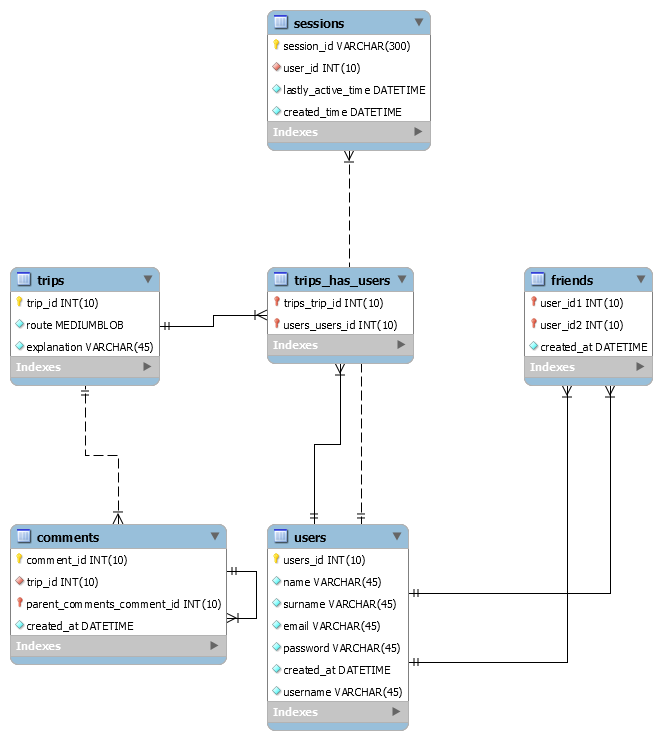
\includegraphics[width=\textwidth]{projectChapters/images/databaseDesign.png}
\caption{Backend Database design
 pattern}
 \label{fig:dbdesign}
\end{figure}
 
\newpage

\begin{figure}[!htbp]
\centering
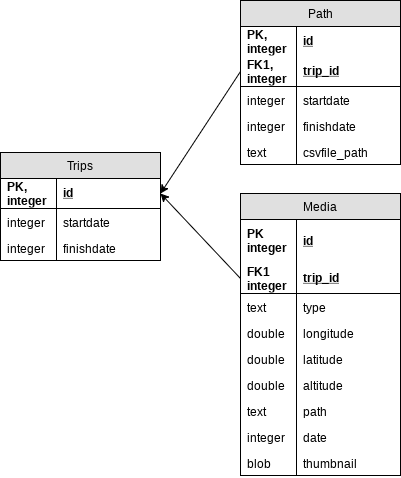
\includegraphics[width=\textwidth]{projectChapters/images/android_database.png}
\caption{Mobile Application Database Diagram}
\end{figure} 


\newpage
\section{Software Design}

The modules used in the project and their relationship to entities is shown in Figure \ref{fig:eR}
\begin{figure}[!ht]
\centering
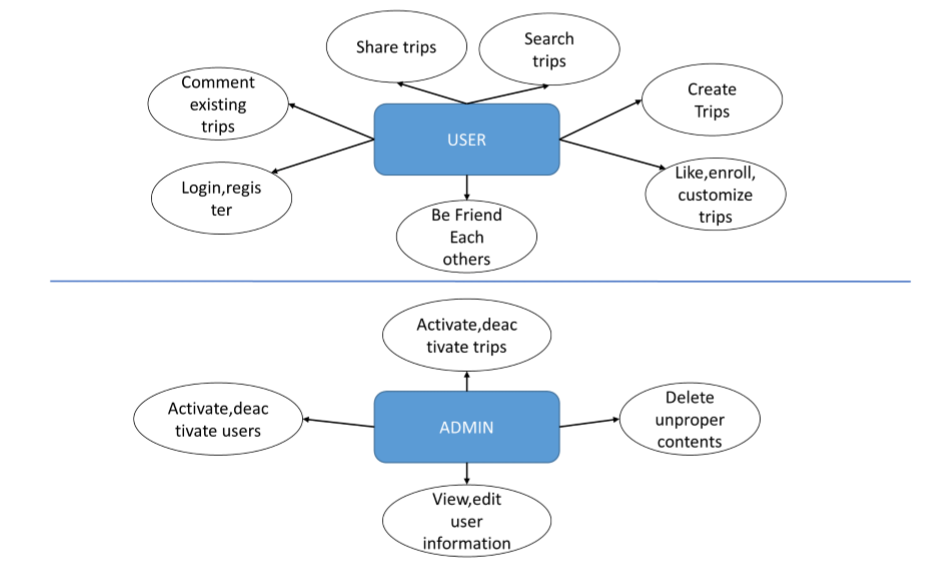
\includegraphics[scale=0.6]{projectChapters/images/ER.png}
\caption{Level zero dataflow diagram }
\label{fig:eR}
\end{figure}


\subsection{User Modules}
\textbf{Create Trips:} Users can create trips by using mobile application.

\textbf{Share Trips:} Users can share trips with their friends or anyone who they like to see or interact with their sharings. 

\textbf{Search trips:} Users can search trips which has been created other users.


\textbf{Like,enrol,customize trip:} Users can like shared trips. They can enrol them by meaning enrolling they can download trips they want in their local storage and view it whenever they want also they can modify the shared trips which lets them to see the content only they preferred.

\textbf{Be each others friends:} Users can be friends each other through web site and mobile application. By doing this they give permission the ones to see their shared trips which is only open to their friend

\textbf{Login and register:} Users can log in or log out to the system.

\textbf{Comment existing trips:} Users can comment on trips that have been shared by other users, they also can attach other users to their comment.

\subsection{Administrator Modules}
\textbf{Evaluate complaints:} Administrators are able to hide or not hide and close complaints by looking its content.

\newpage
The dataflow diagrams of the system are shown in Figure \ref{fig:dataflow}, \ref{fig:dataflow2}, \ref{fig:dataflow3} and \ref{fig:dataflow4}.
\newline
These diagrams give information about the general operation of the system.
\begin{figure}[!ht]
\centering
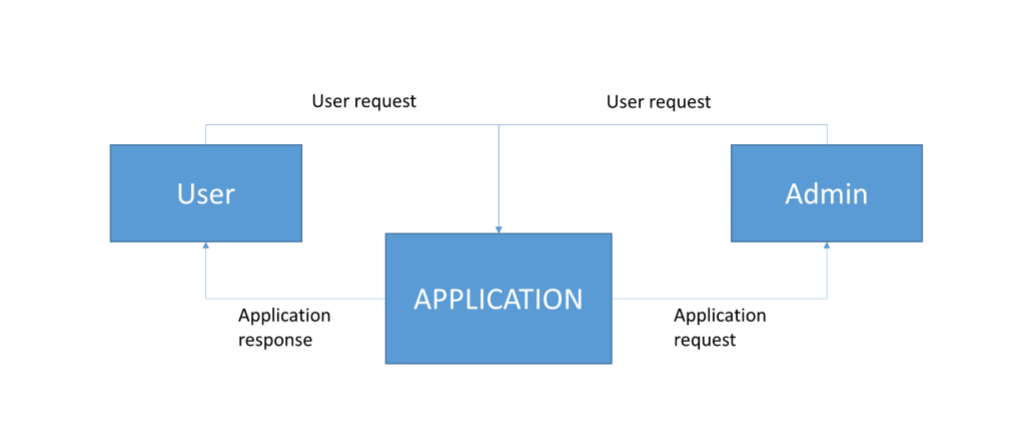
\includegraphics[scale=0.6]{projectChapters/images/dataflow.png}
\caption{Level zero dataflow diagram }
\label{fig:dataflow}
\end{figure}

\begin{figure}[!ht]
\centering
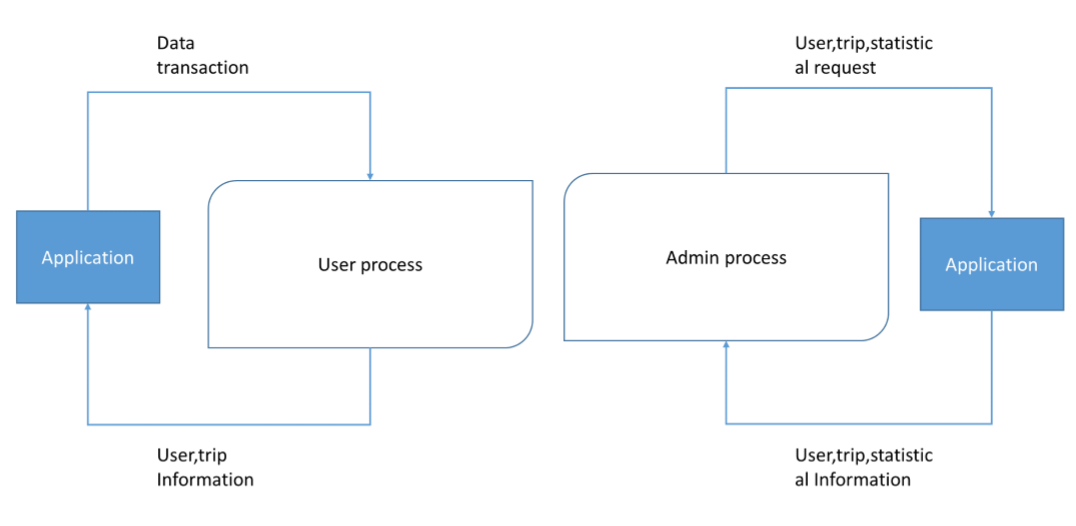
\includegraphics[scale=0.6]{projectChapters/images/dataflow2.png}
\caption{Level one dataflow diagram}
\label{fig:dataflow2}
\end{figure}

\begin{figure}[!ht]
\centering
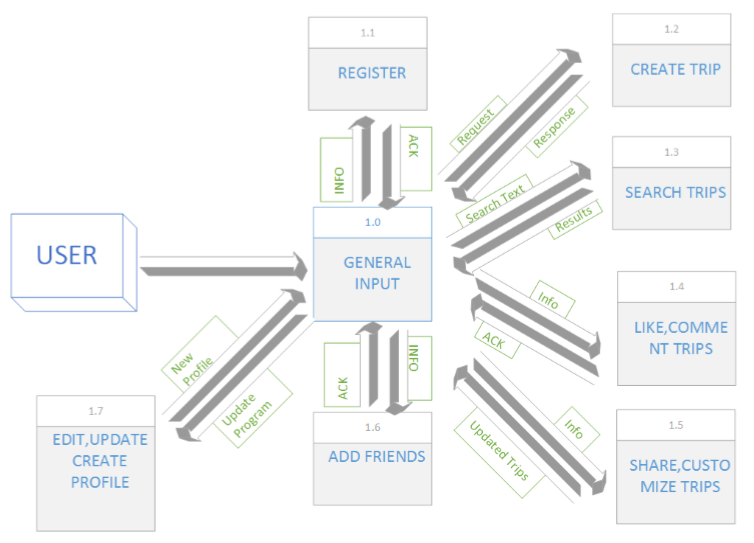
\includegraphics[scale=0.6]{projectChapters/images/dataflow3.png}
\caption{Level two user dataflow diagram}
\label{fig:dataflow3}
\end{figure}

\begin{figure}[!ht]
\centering
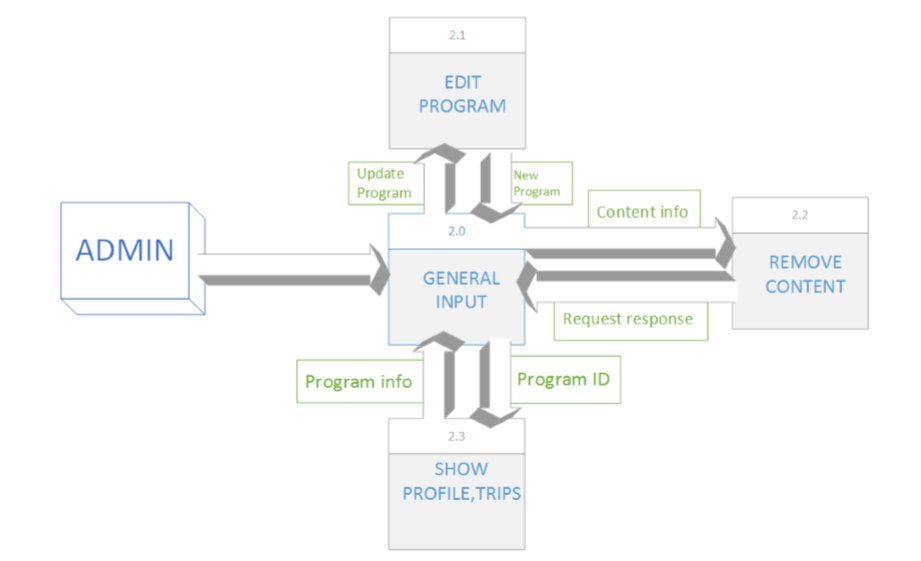
\includegraphics[scale=0.6]{projectChapters/images/dataflow4.png}
\caption{Level two administrator data flow diagram}
\label{fig:dataflow4}
\end{figure}






